%%%%%%%%%%%%%%%%%%%%%%%%%%%%%%%%%%%%%%%%%%%%%%%%%%%%%%
%
% This file defines the style for your report.
%
% Just run "sh compiletex.sh" to compile
% 
%%%%%%%%%%%%%%%%%%%%%%%%%%%%%%%%%%%%%%%%%%%%%%%%%%%%%%

\documentclass[10pt,  english, makeidx, a4paper, titlepage, oneside]{book}
\usepackage{babel}
\usepackage{fancyhdr}
\usepackage{makeidx}
\usepackage{titlesec}
\usepackage{listings}
\usepackage{booktabs}
\usepackage{hyperref}

\newenvironment{listato}{\footnotesize}{\normalsize }

\textwidth 15.5cm
\textheight 23cm
\topmargin -1cm
\oddsidemargin -0.5cm
\linespread{1.1}

\pagestyle{fancy}
\lhead{}
\chead{Cybersecurity for Embedded Systems}
\lfoot{}
\cfoot{}
\rfoot{}
\rhead{\thepage}

\usepackage{graphicx}
\usepackage{amsmath}
\usepackage{amsfonts}
\usepackage{amsthm}
\usepackage{amssymb}
\usepackage{graphicx}
\usepackage{caption}
\usepackage{float}
\usepackage{amsmath}
\usepackage{amssymb}
\usepackage{amsfonts}
\usepackage{amsthm}
\usepackage{empheq}
\usepackage{verbatim}
\usepackage{fancyvrb}
\usepackage{xcolor}

\titleformat{\chapter}[display]
{\normalfont\Large\filcenter\sffamily}
{\titlerule[0.5pt]%
\vspace{1pt}
\titlerule
\vspace{1pc}
\LARGE\MakeUppercase{\chaptertitlename} \thechapter
}
{1pc}
{\titlerule
\vspace{1pc}
\Huge}

\makeindex

\begin{document}

\frontmatter
\begin{titlepage}
    \vspace{0cm}
    \centerline{
        
\includegraphics[width=6cm]{./logopolitonuovo}}
    \vspace{0.5cm}
    \centerline{\LARGE Politecnico di Torino}
    \vspace{2.5cm}
    \centerline{\huge Cybersecurity for Embedded Systems}
    \vspace{0.25cm}
    \centerline{\huge 01UDNOV}
    \vspace{1cm}
    \centerline{\Large Master's Degree in Computer Engineering}
    \vspace{2.5cm}
    \centerline{\Huge Track 2: DoS attacks on microphones}
    \bigskip
    \centerline{\huge Project Report}
    \vspace{2cm}
    \vfill
    \begin{minipage}{7.5cm} % modify this width in order to keep everything on the same line
        \Large{Candidates:\\
            Costabile Digregorio (S318078)\\
            Francesco Gallo (S319989)\\
            Gianmarco Bachiorrini (S309909)}
    \end{minipage}
    \hfill
    \begin{minipage}{5.5 cm}
        \Large{Referee: \\
            Prof.  Alessandro Savino \\}
    \end{minipage}
\end{titlepage}

\tableofcontents
\listoffigures % REMOVE THIS IF THERE ARE NO PICTURES
\listoftables % REMOVE THIS IF THERE ARE NO TABLES

\mainmatter

% HERE IS WHERE YOU INCLUDE YOUR CHAPTERS

\chapter*{Abstract}
The rapid growth of IoT devices in recent years has shaped everyday life more profoundly than most technological advancements in history. 
As with any widespread innovation, this global adoption brings both benefits and drawbacks. 
The conveniences introduced by IoT and smart devices are now integral to modern life, making them difficult for society to forgo. 
However, the rising number of these devices also opens up more potential attack surfaces for malicious actors. 
When considering that many of these devices accompany individuals nearly constantly, the threat to personal privacy rises substantially.

This project focuses on one specific aspect of the problem: its objective is to prevent the unauthorized recording of sensitive conversations through microphones.
The selected methodology to achieve the objective is to execute a Denial of Service (DoS) attack on the microphones by overwhelming them with ultrasonic sound waves.
To demonstrate the effectiveness of this method, a fully functional prototype device capable of executing the attack has been developed.

This report provides a detailed explanation of each step in the development process, starting with the analysis of microphone technologies and a review of state-of-the-art attacks targeting them, followed by the formulation of the core concept, and concluding with its final implementation.
To facilitate a deeper understanding of its functionality, the report includes a comprehensive explanation of each component and of the source code.

The prototype device has been thoroughly tested on the most common types of devices, including smartphones, PCs, and smartwatches, across various distance ranges, and has demonstrated highly promising results.
The reports concludes with an analysis of the known issues and of the areas that could be furtherly improved in the future in order to deliver a product even more effective, reliable and feature-rich.
%\chapter{Generic Chapter}
This is a generic chapter of your thesis. Remember to put ANY chapter in a different source file (including introduction and all the others).

For the purpose of this guide, the main \LaTeX constructs and how to use them will be explained here. Other thematic chapters will follow, i.e., which will trace the chapters that should be present in your thesis. Delete this generic chapter once you have learned this contents.

You can write in italic \emph{like this}, you can write in bold \textbf{like this}, or you can write using colors \textcolor{cyan}{like this}.

This is an \emph{itemize}, where you can put a list of items, like this:
\begin{itemize}
	\item item number 1
	\item item number 2
\end{itemize}

This is an \emph{enumerate}, where you can put a list of items with numbers, like this:
\begin{enumerate}
	\item item number 1
	\item item number 2
\end{enumerate}

You can cite references like this: \cite{texbook} \cite{lamport94}, by using the \lstinline{\cite} directive. You have to copy within \lstinline{\cite} brackets the label of the entry that you have in the BibTeX file (\texttt{.bib}). The \texttt{.bib} file of this thesis is \texttt{mybib.bib}. he command \lstinline{\addbibresource} at the top of this main file indicates what BibTeX file you are referring to.

As an example, this is a BibTeX entry:

\begin{verbatim}
@inproceedings{urias2018cyber,
  title={Cyber Range Infrastructure Limitations and Needs of Tomorrow: A Position Paper},
  author={Urias, Vincent E and Stout, William MS and Van Leeuwen, Brian and Lin, Han},
  booktitle={2018 International Carnahan Conference on Security Technology (ICCST)},
  pages={1--5},
  year={2018},
  organization={IEEE}
}
\end{verbatim}

For every online paper that you may read on online libraries, you can download its BibTeX entry. For example:
\begin{enumerate}
	\item For IEEE Xplore, click on the paper name, then click on ``Cite This'', ``BibTeX'', and you can find the entry;
	\item For Google Scholar, click on the ``Cite'' voice under the paper name, then click ``BibTeX'', and you can find the entry.
\end{enumerate}

Just copy and paste such an entry in the .bib file. If you find a paper on Scholar that is nevertheless published by IEEE, by convention you should take the entry from the IEEE website and not from Scholar. To do this, just click on the title of the paper. This will redirect you to the resource page on IEEE Xplore. Once here, follow instructions at point 1.

When you compile, a correct number will automatically be assigned to the citation in the text, and the complete entry will appear at the bottom of the document, in the ``Bibliography'' chapter.

If you need to cite a generic online resource, which does not necessarily correspond to a scientific paper, use the \lstinline{@misc} entry in the \texttt{.bib} file. A \lstinline{@misc} entry looks like this:

\begin{verbatim}
@misc{nist2018,
    author = "{NIST}",
    title = "Cyber Ranges",
    year = "2018",
    howpublished = "\url{https://www.nist.gov/system/files/documents/2018/02/13/cyber_ranges.pdf}",
    note = "[Online; Accessed 2019, 28 November]"
  }
\end{verbatim}

You have to manually create this entry from scratch and manually type these fields. Remember not to forget any of these fields. You can choose the label with which to refer to the resource. The title of the website (which you can see at the top of the tab of your browser showing the page) can be used as the title of the resource.

In general, enter a citation of this type for sites only when there are data, phrases, or images that you intend to report. Instead, if you want to cite names of software or hardware devices, prefer the use of the \lstinline{\footnote}, in which you will only have to specify the URL of the item.

Remember that citations, both in the text and in the image captions, usually go to the end of a sentence, before the fullstop, as in this case \cite{vykopal2017kypo}. In case of long periods, they can also be placed before other detachment signs, such as commas or semicolons, or colons if they precede a list, itemized or enumerated. An exemption is allowed in the event that the name of research projects, described in some scientific resource, is being introduced, as in this case:

\begin{center}
	Cybertropolis \cite{deckard2018cybertropolis} is described in a very good paper by Gary Deckard.
\end{center}

Remember to put citations very often to justify your claims, especially when you report data or results. Just consider them as a justification of what you, in an original way, are writing. Citations are not needed to have permission to copy and paste sentences from online resources, which should NEVER be done - always try to rephrase the concept with your words.

\begin{figure}[h!]
	\vspace{0.5cm}
	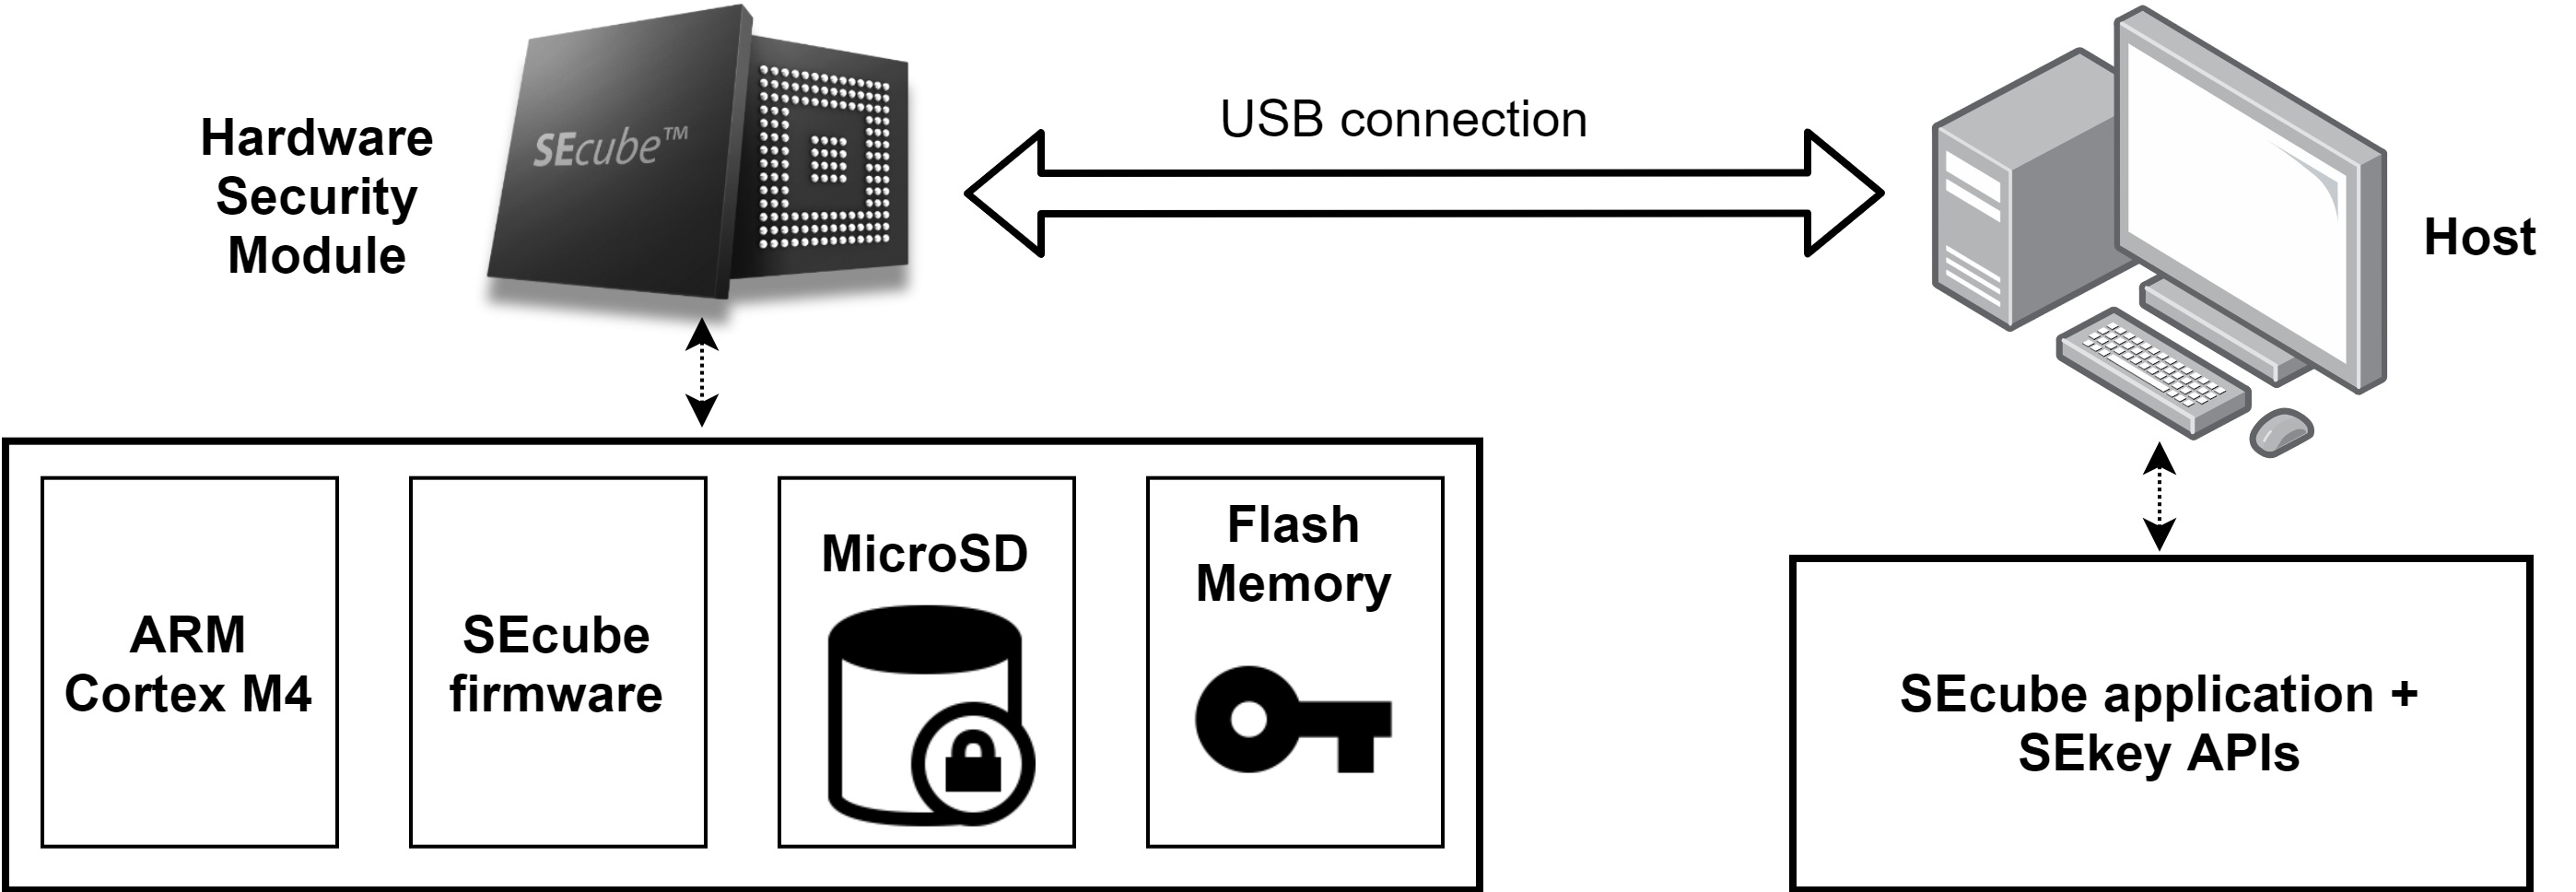
\includegraphics[width=\textwidth]{images/simplearch.jpg}
	\caption{This is the image \emph{caption}.}
	\label{fig:generalschema} % This is the image label, with which you can refer to the image in any document location.
\end{figure}

This is an image example. Images must ALWAYS be understandable: never introduce images that have text smaller than the text in your document. If you create the images yourself, try not to make them clash too much with the style of your document, and use the same font as this thesis.
If they are not images of your own creation, you MUST reference them. In the caption of the image, you need to insert a citation to the resource from which you took the image, at the end of the caption sentence, before the fullstop.
Each image you enter MUST be referenced in the text, using a formula similar to this:

\begin{center}
	Figure \ref{fig:generalschema} describes the architecture of the system.
\end{center}

You can refer to the image using \lstinline{\ref} followed by the image label, that you put in the \lstinline{\label} entry of the figure. Remember to use the word Figure with a capital F.

Remember that the more your text is adorned with figures, the more understandable, appreciable and readable it becomes.

\section{Section title}\label{examplesection}
This is a section under a chapter. The number of sections also contributes to greater readability of your text, and to a better display of the content in the index. In fact, sections are automatically shown in the Table of Contents. However, try not to make sections shorter than two pages. For smaller portions of your text, use subsections.

You can refer to a section using its label, using the \lstinline{\ref} directive as for images, like this:

\begin{center}
	This concept has been explained in Section \ref{examplesection}.
\end{center}

Remember to use the word Section with a capital S. This is also valid for chapters.

\subsection{Subsection title}
This is a subsection under the section.

The following is a table.

\begin{table}
	\centering
	\caption{Preliminary Experimental Results}
	\begin{tabular}{| p{3cm} | p{3cm} | p{3cm} |}
		\hline
		\textbf{Benchmark} & \textbf{Inputs}                   & \textbf{Processing time} \\ \hline
		SHA                & Message of 100 KB                 & 368449 s                 \\ \hline
		RIJNDAEL           & Message of 100 KB                 & 1083568 s                \\ \hline
		DIJKSTRA           & Matrix of 100x100 32-bit integers & 324782 s                 \\ \hline
		STRING             & 1331 50-char strings              & 178616 s                 \\ \hline
		BITCOUNT           & 12800 32-bit integers             & 419545 s                 \\ \hline
		\hline
	\end{tabular}
	\label{tab:ar}
\end{table}

If you want to write a formula, you can do like this:

\begin{equation}\label{eq:thiseq}
	X_{k}=\sum _{n=0}^{N-1}x_{n}e^{-ik{\frac {2\pi }{N}}n}\quad \quad k=0,\dots ,N-1
\end{equation}

Tables and formulas are extensively documented online, and any doubts about their syntax can be easily resolved with a simple search. As for figures and sections, the same rules also apply to tables and formulas: mandatory reference in the text, possibility to use \lstinline{\label} to label them, and naming with capital letter (e.g., ``as in Table \ref{tab:ar}, as in Formula \ref{eq:thiseq}).

The following is a piece of code:

\begin{lstlisting}
int func(int N, int M) {
  float (*p)[N][M] = malloc(sizeof *p);
  if (!p)
    return -1;
  for (int i = 0; i < N; i++)
    for (int j = 0; j < M; j++)
      (*p)[i][j] = i + j;
  print_array(N, M, p);
  free(p);
  return 1;
}
\end{lstlisting}

You can customize the style of your code, changing the language, the colors of keywords, of comments or the background by changing the settings inside the \lstinline{\lstset} directive found in the main file. Usually, the listings are not referenced within the text as happens for figures, tables, formulas and sections. Do not overdo the code within your text: use it only for short passages (e.g., function prototypes, or 2 to 5 lines of code within a function to help the reader in better understanding the meaning of the text).

You can also write in-text code using the \lstinline{\lstinline} directive, \\
like this: \lstinline{int main(int argc, char** argv);}.




\chapter{Introduction}
\section{Report introduction}
In recent years, there has been a rapid proliferation of devices equipped with microphones, such as smartphones, smart speakers, and smartwatches.
This has led to a significant decline in user privacy, especially as many of these devices come with an 'always-listening' feature enabled by default.
As a result, the security vulnerabilities in microphones have attracted the attention of both attackers and defenders: while the motivations of the former are self-evident, the latter, in an interesting role reversal, can leverage these vulnerabilities to enhance user privacy.
In other words, it is possible to execute an attack that disables nearby microphones to preserve the privacy of users who may be unaware of potential eavesdropping.

From the perspective of improving user privacy by exploiting microphones' vulnerabilities, this project investigates Denial of Service (DoS) attacks on microphones, with the goal of understanding the underlying technologies, identifying vulnerabilities, and replicating attacks on real hardware.
The project seeks to provide a comprehensive analysis of microphone manufacturing technologies, evaluate the state-of-the-art in attack techniques, and explore the limitations and implications of these attacks.
In particular, the project will focus on a specific type of DoS attack, which involves flooding the target microphone with ultrasound waves to prevent it from recording any conversation.
Additionally, a fully functioning prototype device capable of executing the attack has been developed.
As we navigate through both the sotware and hardware implementations of the project, an analysis of the results will be presented, assessing the strengths and weaknesses of the prototype device.

\section{Report description}
The remainder of the document is organized as follows:
\begin{itemize}
    \item Chapter 2: This chapter offers a comprehensive overview of the project's theoretical background, detailing the key features of various microphone technologies and examining known attack methods.
    \item Chapter 3: This chapter provide a general overview of the project's implementation, offering the reader a simple description of the prototype device's components and capabilities.
    \item Chapter 4: This chapter presents a detailed explanation of the device, covering everything from its initial design to its physical construction and realization.
    \item Chapter 5: This chapter outlines the results obtained and proposes ideas for potential improvements to the device in future work.
    \item Chapter 6: This chapter recaps with a high-level summary what has been done in the project.
\end{itemize}


\chapter{Background}
This section of the report will introduce to the reader the most relevant microphone technologies, highlighting their core features and primary domains of use.\\
Furthermore, the different types of known DoS attacks on microphones will be reviewed, evaluating the advantages and disadvantages of each. This analysis will justify the selection of the chosen attack method for the project.
\section{Microphone Technologies}
Microphones are critical components in many modern devices, enabling audio capture for communication, recording, and interaction with digital assistants.
Since they are used in a wide range of devices, their underlying technology must meet diverse requirements, resulting in both orizontal diversification and vertical improvement over the past century.\\
While acknowledging the historical significance of early microphone implementations, this report will focus only on the most commonly used models today, as they are most relevant to the development of the project.
\subsection{Dynamic Microphones}
A dynamic microphone is a type of mic that converts sound waves into electrical signals using electromagnetic induction thanks to a special component, the permanent magnet.
The permament magnet can either be a metal coil or a 'ribbon transducer': when the sound waves hit the microphone, the magnet will move, resulting in the generation of an electrical signal.
This type of microphone is known for its durability, ability to handle loud environments, and tolerance of background noise.
Additionally, it does not require external power, making it a versatile option for various situations.
Although it may not be as sensitive or well-suited for recording high-frequency sounds, it is ideal for live music events and concerts involving loud sounds.
\subsection{Condenser Microphones}
Often referred to as the 'cousins' of dynamic microphones, condenser microphones generate electrical signals from sound waves through the use of a capacitor.
The capacitor consists of two charged metal plates, one of which is movable.
When a sound wave strikes the diaphragm (the movable plate), the distance between the plates changes, producing an electrical signal that corresponds to the sound captured.
While condenser microphones require an electrical current to charge the plates and are more sensitive to environmental conditions compared to dynamic microphones, they excel at capturing high-frequency sounds and vocals, delivering crisp, detailed, and high-quality audio.
These qualities make condenser microphones ideal for studio recording, as they are best suited for quiet environments and require the external power source.
\subsection{Electret Condenser Microphones}
The electret condenser microphone is a subtype of the standard condenser microphone.
The key difference is that, while standard condenser microphones require a power supply to maintain the electrical charge, electret microphones use an electret material to keep the capsule charged.
This type of material is one that carries a permanent electrical charge sealed within an insulating film.
Since electret microphones don’t require an external power source to charge the plates, they tend to be less expensive than standard condenser microphones, making them ideal for use in consumer electronics and mobile devices.
\subsection{Micro-Electro-Mechanical Systems Microphones}
MEMS microphones is another subtype of the standard condenser microphone which shares many characteristics with the electret type one.
However, in this case, the transducer is a microscopic component that integrates seamlessly with the microscopic semiconductor-based components in an integrated circuit.
This allows for smaller devices, making them suitable for an even wider range of applications, such as smartphones, tablets, laptops, hearing aids, voice biometric, digital voice assistants, and more.
Additionally, compared to electret microphones, MEMS microphones can offer superior audio performance, though they tend to be more susceptible to mechanical and electrical noise.

\section{Microphone Attacks}
Having explored the landscape of microphone technologies, it is evident that the ones we encounter most frequently in daily life are Electret microphones, and even more commonly, MEMS microphones.
Both technologies share key components, namely the membrane and the capacitor, each of which is vulnerable to specific types of attacks that can effectively prevent microphones from recording conversations intended to remain private. \\
The membrane can be made to vibrate by flooding the microphone with sound waves, thereby overwriting the sound waves from the conversation and preventing proper recording.
Meanwhile, the capacitor can be targeted by altering its electric charge, causing it to produce a distorted or different electrical signal instead of the original one.\\
The following section will examine known DoS attacks that exploit the vulnerabilities of these two components, evaluating each attack technique in terms of its suitability for the project.
\subsection{Electromagnetic Pulse Attack}
A general EMP attack involves releasing a burst of electromagnetic radiation capable of disrupting or destroying electronic equipment and systems across the target area.
It is frequently employed in modern warfare with the goal of causing infrastructural disruption, targeting communication systems, computers, vehicles, and other critical equipment.\\
When using an EMP to disable microphones, the strategy involves emitting a powerful burst of electromagnetic radiation that overwhelms and potentially damages the electronic components within the microphones.
This could result in the microphones failing to generate the intended electrical signals, or even becoming completely non-functional, thus disabling their ability to record or transmit audio.
The severity of the impact would depend on the intensity and proximity of the EMP, potentially leaving affected microphones unusable until they are repaired or replaced.\\
While theoretically the most effective method on paper, employing an EMP for this project is impractical for several reasons.
First and foremost, health concerns must be taken into account, as this type of attack could pose risks to nearby individuals with pacemakers, hearing aids, or other medical devices.
Secondly, it would lack control over the range of action and the potential impact on targets.
Additionally, testing the prototype device would be extremely difficult, with results that could be highly unpredictable and the testing targets potentially suffering permanent damage.
Finally, the need for high power sources makes it unsuitable for embedded devices.
\subsection{Laser Injection Attack}
Luminous attacks on microphones involve using lasers to disrupt or damage their functionality.
Lasers emit focused beams of intense light that can interfere with microphones in several ways.
First, a powerful laser beam can overload the microphone's optical or electronic sensors, causing them to register false signals.
Second, laser light can interfere with the microphone's ability to accurately capture sound waves, potentially distorting or disrupting the audio signal.
In extreme cases, particularly with high-powered lasers, the intense heat generated by the beam can physically damage the microphone's components, such as diaphragms, sensors and circuitry.
Moreover, luminous attacks can compromise privacy by remotely activating microphones through light-based signals, thereby bypassing traditional security measures. \\
However, this type of attack does not align with the project's objectives.
The limited applicability due to its high specificity, the need for precise targeting making it impractical in general environments, and its high production costs classify the laser injection attack as unsuitable for this project.
\subsection{Ultrasonic Sound Waves Jamming Attack}
Ultrasonic sound waves are those that travel at frequencies above 20 kHz, exceeding the range of human hearing.
This type of sound wave can be used to perform jamming attacks on microphones, disrupting their functionality.
In particular, they can overwhelm the microphone's sensors, which are typically calibrated to capture frequencies within the audible spectrum.
When exposed to ultrasonic sound waves, these sensors may register false signals or become saturated, resulting in inaccurate audio captures and, thereby, distorted or unintelligible audio output. \\
This attack meets all the requirements to be suitable for the project: it can target nearly any everyday microphone, delivers strong performance, and when properly tuned, becomes extremely difficult—if not impossible—for humans to detect.
Moreover, its low implementation cost and non-destructive nature make testing the prototype device much more feasible.
\chapter{Implementation Overview}
This chapter presents the project's objectives, the specific problem it seeks to address, and the challenges encountered during its development. 
Additionally, it provides a high-level overview of the proposed solution.

\section{Goal of the project}
Nowadays, with the rise of smart devices and the increasing spread of home automation, we are literally surrounded by microphones.
All these devices can potentially be used to record sensitive data from our conversations without our consent.

The goal of this project is to create a device capable of (at least partially) deny the aforementioned risk and enhance users' privacy.
The desired device should satisfy the following requirements:
\begin{itemize}
    \item Effectiveness: the device should deliver perceptually high performance within a reasonable operational range.
    \item Inaudibility to humans: the device should operate without causing any disturbance during conversations and should only interfere with the functionality of microphones when activated.
    \item Portability: the device should be designed to be easily transportable.
    \item Ease of use: the device should be intuitive and user-friendly, ensuring that it can be operated by individuals of varying technical expertise.
    \item Low energy consumption: the device should be designed to operate with minimal energy requirements.
    \item Affordability: the device should be produced at minimal cost while ensuring all required functionalities are maintained.
\end{itemize}
If all the requirements are met, the device will offer an effective solution to the problem, enhancing the privacy of individuals who are often concerned about the risk of being recorded.

\section{Core Concept}
The first step is to formalize the problem and identify the most suitable attack vector that meets the previously aforementioned requirements.
Following a thorough analysis, as outlined in \nameref{background}, the ultrasonic sound wave jamming attack was determined to be the most appropriate option due to its high applicability, (potential) strong performance, and difficulty for humans to detect.

A cost-effective implementation of this attack involves the use of ultrasonic transducers, which are commonly found in low-cost distance sensors as they operate at the required frequencies (above 20kHz), or they can be bought in bundle at almost any online electronic retailer.
Consequently, a signal generator is required to produce the appropriate sound wave for the speaker. 
Finally, a microcontroller is necessary to orchestrate the operation of the device, managing the control logic and interfacing with the signal generator. 

\section{Key Challenges in Implementing the Core Concept}
The core concept satisfies certain requirements, such as inaudibility to humans and low cost. 
However, aspects like portability, effectiveness, and ease of use are not fully achieved by implementing only the core idea. 
Furthermore, some properties are inherently interconnected. 
For example, increasing effectiveness may raise overall costs, reducing affordability, while portability is closely tied to low energy consumption, as high energy demands would compromise the device's practicality.

Therefore, careful evaluation and selection of available market components are crucial to ensure all requirements are met.

\section{Practical Implementation of the Core Concept}
Having outlined the core concept, its development requires additional components to ensure full functionality and satisfy the imposed requirements. 

To make the signal effective in a real-world scenario, an audio amplifier is necessary, as the generated signal's power must be boosted to a specific level.
By utilizing an external power source, the amplifier module interfaces the microcontroller-signal generator subsystem with the speaker.

The external power source has been implemented as a set of batteries to ensure portability and keep costs low.
Specifically, the batteries are lithium-based and are connected together to achieve the required voltage and power.

Finally, a remote-controlled switch has been integrated, enabling the end user to power the device on and off via the \textit{Home} application in the iOS environment or through the lightweight MQTT protocol.

\section{Final Implementation}
At this stage, with all functional and non-functional requirements met through the selected components, the final step is to design the device and integrate all elements into a cohesive unit.

The speakers are embedded into a 3D-printed spherical shell with strategically placed openings to house them. 
This design enables the jamming attack to be performed in nearly a 360-degree radius, maximizing the coverage of the surrounding area.
\begin{figure}[H]
    \centering
    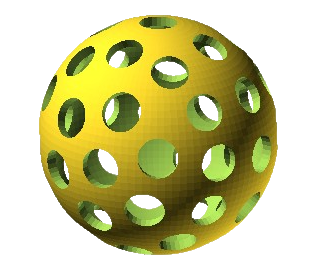
\includegraphics[width=0.25\linewidth]{images/image-removebg-preview.png}
    \caption{3D-printed spherical shell}
\end{figure}
The shell is mounted on a base that houses the battery along with all the previously mentioned components, including the microcontroller, audio amplifier module, signal generator, and remote-controlled switch. 
This base provides an organized and concealed arrangement of the internal components, offering the end user a polished and minimalist appearance while maintaining practicality.
\begin{figure}[H]
    \centering
    \begin{subfigure}[b]{0.4\linewidth}
        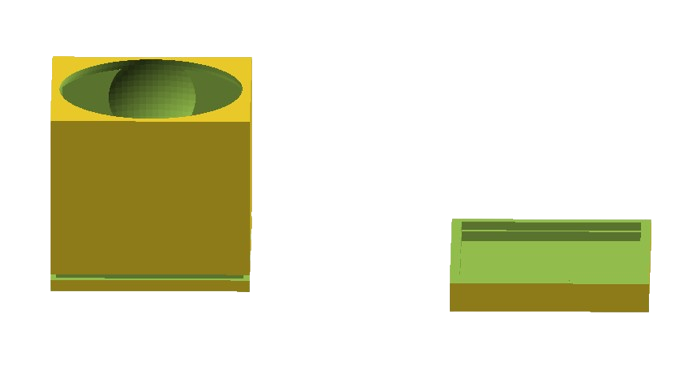
\includegraphics[width=\linewidth]{images/Supports.png}
        \caption{Support base}
    \end{subfigure}
    \begin{subfigure}[b]{0.4\linewidth}
        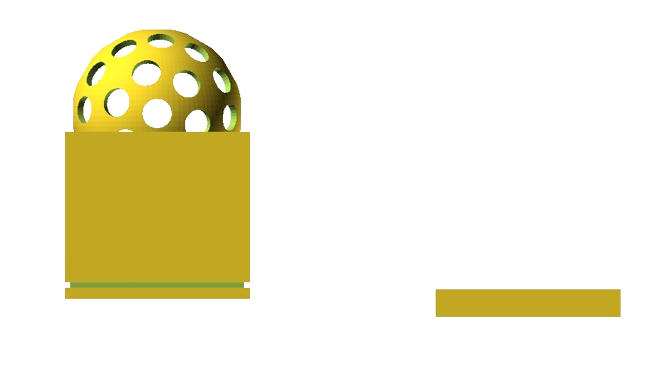
\includegraphics[width=\linewidth]{images/Jammer+Supports.png}
        \caption{Shell resting on the base}
    \end{subfigure}
    \caption{Final implementation appearance}
\end{figure}

\chapter{Implementation Details Template}
This is where you explain what you have implemented and how you have implemented it. Place here all the details that you consider important, organize the chapter in sections and subsections to explain the development and your workflow.\\Given the self-explicative title of the chapter, readers usually skip it. This is ok, because this entire chapter is simply meant to describe the details of your work so that people that are very interested (such as people who have to evaluate your work or people who have to build something more complex starting from what you did) can fully understand what you developed or implemented.\\Don't worry about placing too many details in this chapter, the only essential thing is that you keep everything tidy, without mixing too much information (so make use of sections, subsections, lists, etc.). As usual, pictures are helpful.
\chapter{Implementation Details}

\section{Overview}
In questa sezione viene fornita una panoramica generale dell'implementazione del jammer di microfoni. L'obiettivo del progetto è stato quello di disturbare i microfoni utilizzando segnali ultrasonici generati da un sistema controllato da remoto tramite Apple Home e MQTT. Di seguito sono dettagliate tutte le fasi di sviluppo, dall'hardware al software, fino alla progettazione 3D e all'integrazione finale.
In that section we will provide a detailed explanation of the implementation of the microphone jammer. The project aimed to disrupt microphones using ultrasonic signals generated by a system remotely controlled via Apple Home and MQTT.
Below are detailed all the development phases, from hardware to software, to 3D design and final integration.


\section{Hardware Setup}

\subsection{Microcontroller - Arduino Uno}
An Arduino Uno microcontroller was used to manage the system. Arduino was chosen for its ease of use and flexibility, allowing it to interface with a wide range of hardware devices. 
Below are its key technical specifications:
\begin{itemize}
    \item \textbf{Microcontroller}: ATmega328P
    \item \textbf{Operating Voltage}: 5V
    \item \textbf{Input Voltage (recommended)}: 7-12V
    \item \textbf{Input Voltage (limit)}: 6-20V
    \item \textbf{Digital I/O Pins}: 14 (6 PWM outputs)
    \item \textbf{Analog Input Pins}: 6
    \item \textbf{DC Current per I/O Pin}: 20 mA
    \item \textbf{DC Current for 3.3V Pin}: 50 mA
    \item \textbf{Flash Memory}: 32 KB (0.5 KB used by bootloader)
    \item \textbf{SRAM}: 2 KB
    \item \textbf{EEPROM}: 1 KB
    \item \textbf{Clock Speed}: 16 MHz
    \item \textbf{Interfaces}: UART, SPI, I2C
\end{itemize}
The microcontroller was employed to control the signal generator, ensuring it produced the desired waveform at the required frequency. 

\subsection{Signal Generator - AD9833}

The \textbf{AD9833} signal generator was utilized in this project to produce the ultrasonic signals required to interfere with microphones. The AD9833 is a highly versatile, low-power, programmable waveform generator that can generate \textit{sine}, \textit{triangle}, and \textit{square wave} outputs over a wide frequency range. It employs a \textbf{numerically controlled oscillator (NCO)} to ensure precise frequency generation with minimal drift, making it ideal for applications requiring stable and accurate signal production.

Key features of the AD9833 include:

\begin{itemize}
    \item \textbf{Frequency Range}: The AD9833 is capable of generating waveforms from near-DC to several MHz. In this project, it was configured to output signals in the ultrasonic range, specifically between $24 kHz$ up to $26 kHz$.
    
    \item \textbf{Low Power Consumption}: With typical power consumption of $20 mW$, the AD9833 is well-suited for battery-powered applications. Its energy efficiency made it an ideal choice for the portable jammer system developed in this project.
    
    \item \textbf{Waveform Generation}: The AD9833 can produce \textit{sine}, \textit{triangle}, and \textit{square waves}, providing flexibility in signal generation. For this project, the \textit{square wave output} was selected due to its efficiency in driving the ultrasonic transducers and maximizing interference with microphone diaphragms.
    
    \item \textbf{Programmability}: The output frequency and waveform type of the AD9833 are fully programmable via the \textbf{SPI (Serial Peripheral Interface)}. This programmability allows dynamic adjustments of the ultrasonic signal, facilitating quick testing of different frequencies to identify the optimal one for microphone disruption.
    
    \item \textbf{Compact Size}: The AD9833 is available in a small \textit{10-lead MSOP package}, which makes it ideal for compact designs. Its size made it well-suited for the jammer system, where space was limited.
\end{itemize}

In this implementation, the AD9833 was controlled by an Arduino through the SPI interface, with the output waveform subsequently amplified and transmitted via ultrasonic transducers. This configuration allowed for precise generation of high-frequency signals that were capable of effectively disrupting nearby microphones.

\subsection{SPI Communication Protocol}

The AD9833 programmable waveform generator communicates with the Arduino Uno using the SPI (Serial Peripheral Interface) protocol. SPI is a synchronous serial communication protocol commonly used to exchange data between a master device (in this case, the Arduino) and one or more slave devices (such as the AD9833). The protocol is fast and efficient, utilizing four main signals:

\begin{itemize}
    \item \textbf{MOSI (Master Out Slave In)}: Sends data from the master (Arduino) to the slave (AD9833).
    \item \textbf{MISO (Master In Slave Out)}: Receives data from the slave. (Not used in this specific application with the AD9833.)
    \item \textbf{SCLK (Serial Clock)}: Synchronizes the communication by generating clock pulses.
    \item \textbf{SS/CS (Slave Select/Chip Select)}: Selects which slave device is active for communication.
\end{itemize}

In this project, only three of these signals are needed, as the AD9833 is a write-only device, meaning that it does not send data back to the master.

SPI operates by shifting data in or out of the slave device one bit at a time, synchronized by the clock signal. The data is sent over the \textbf{MOSI} line, with the clock signal driving the data transfer, and the \textbf{SS/CS} line controlling when the slave device (AD9833) is selected for communication.

\subsection{Pin Configuration for AD9833 Communication}

Below are the specific pin configurations used to connect the AD9833 with the Arduino Uno via SPI:

\subsubsection{FSYNC (SS/CS) – Pin 10}
\begin{verbatim}
#define AD9833_FSYNC 10  // PIN SS/CS
\end{verbatim}

The FSYNC pin is assigned to Pin 10 on the Arduino and serves as the \textit{Slave Select (SS)} or \textit{Chip Select (CS)} pin. The FSYNC pin determines when the AD9833 is selected and ready for communication.

\begin{itemize}
    \item When the FSYNC pin is set to \textbf{LOW}, the AD9833 is selected and activated for communication.
    \item When the FSYNC pin is set to \textbf{HIGH}, the AD9833 is deselected and no communication occurs.
\end{itemize}

\subsubsection{SCLK (SCK) – Pin 13}
\begin{verbatim}
#define AD9833_SCLK 13   // PIN SCK
\end{verbatim}

The SCLK pin is defined as the \textit{Serial Clock (SCK)} and is connected to Pin 13 on the Arduino. It generates the clock pulses that synchronize the data transfer between the Arduino and the AD9833.

\begin{itemize}
    \item For every clock pulse on the SCLK line, one bit of data is transmitted or received.
    \item The clock signal ensures that both the Arduino and the AD9833 are synchronized during data transmission.
\end{itemize}

\subsubsection{FDATA (MOSI) – Pin 11}
\begin{verbatim}
#define AD9833_FDATA 11  // PIN MOSI
\end{verbatim}

The FDATA pin is connected to Pin 11 on the Arduino and serves as the \textit{Master Out Slave In (MOSI)} pin. It is used to transmit data from the Arduino to the AD9833.

\begin{itemize}
    \item Configuration data and waveform instructions are transmitted from the Arduino to the AD9833 via the MOSI line.
    \item Data is sent sequentially, one bit at a time, in synchronization with the clock pulses on the SCLK line.
\end{itemize}

\subsection{Summary of Pin Roles in SPI for AD9833}

\begin{itemize}
    \item \textbf{FSYNC (Pin 10)}: Acts as the \textit{Slave Select (SS/CS)} pin to activate or deactivate the AD9833 for communication.
    \item \textbf{SCLK (Pin 13)}: Provides the \textit{Serial Clock (SCK)} signal, ensuring synchronized data transfer between the Arduino and AD9833.
    \item \textbf{FDATA (Pin 11)}: Serves as the \textit{Master Out Slave In (MOSI)} pin, transmitting data from the Arduino to the AD9833.
\end{itemize}

This pin configuration allows precise control of the AD9833 using SPI communication, facilitating the generation of the required waveforms at the desired frequency.

\subsection{Ultrasound Transducers}

The ultrasonic transducers used in this project operate at a frequency of $20 \text{kHz}$, which is beyond the audible range for humans. These transducers are particularly effective for disrupting microphones, as they generate high-frequency sound waves that induce vibrations in the microphone diaphragm, impairing its ability to capture sound accurately.

To maximize the interference effect, the placement and orientation of the transducers are crucial. The transducers should be positioned in close proximity to the target microphones and aligned to ensure the ultrasonic waves are directed precisely at the microphones. One key factor influencing the effectiveness of this interference is the beam angle of the transducers, which defines the spread of the ultrasonic waves.

The beam angle determines how focused or dispersed the sound waves are as they propagate. A narrower beam angle results in a more concentrated sound wave, which can enhance the interference effect over longer distances, while a wider beam angle covers a broader area but with less intensity. Given these considerations, both theoretical and empirical analyses were conducted to identify the optimal arrangement of the transducer array, accounting for beam angle, proximity, and orientation to achieve the most effective disruption of microphone performance.
\begin{figure}[h!]
    \centering
    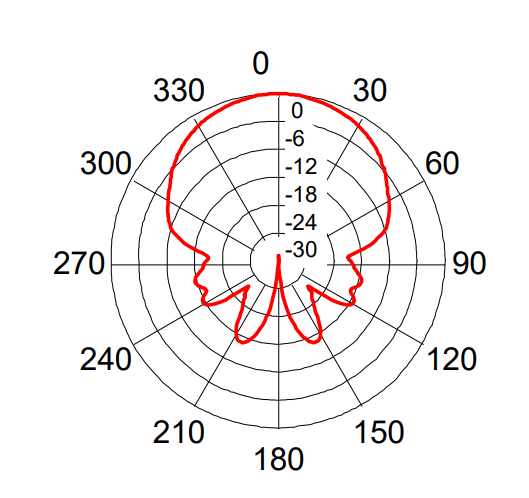
\includegraphics[width=0.5\textwidth]{images/Beam_Angle.png}
    \caption{Beam Angle}
    \label{fig:transducer_shape}
\end{figure}

\subsection{Amplifier - TPA3116D2}

The ultrasonic signals generated by the AD9833, controlled via the Arduino, are amplified using the \textbf{TPA3116D2}, a high-efficiency, Class D audio amplifier from Texas Instruments. The amplifier ensures that the ultrasonic transducers receive a sufficiently powerful signal to produce sound waves with the necessary intensity for effective microphone interference.

The \textbf{TPA3116D2} is specifically designed for high-performance audio applications and is capable of delivering output power of up to \textit{50 W} per channel (with a 4 $\Omega$ load). Key features of the \textbf{TPA3116D2} that make it suitable for this project include:

\begin{itemize}
    \item \textbf{High Efficiency}: The Class D architecture of the amplifier provides high efficiency, with typical values reaching \textit{90\%}. This reduces heat dissipation and ensures lower power consumption, making it well-suited for applications where energy efficiency is critical.
    
    \item \textbf{Output Power}: The TPA3116D2 can deliver up to $50 W$ per channel in stereo mode, or $100 W$ in mono mode. In this project, the amplifier was used to boost the signal to a level that could drive the ultrasonic transducers effectively, ensuring a strong and clear output at the target frequency of \textit{20 kHz}.
    
    \item \textbf{Low Distortion and Noise}: The amplifier features a low distortion rate, typically less than \textit{0.1\% Total Harmonic Distortion + Noise (THD+N)} at full power, ensuring that the signal remains clean. This is crucial for maintaining the integrity of the ultrasonic signal being transmitted to the transducers, as distortion could reduce the effectiveness of the interference.
    
    \item \textbf{Thermal and Overcurrent Protection}: The \textbf{TPA3116D2} includes built-in thermal and overcurrent protection, ensuring reliable operation even under high-power conditions. This feature enhances the robustness of the system, especially when used in a continuous mode, as is typical in ultrasonic jamming applications.
    
    \item \textbf{Wide Supply Voltage Range}: The amplifier operates across a wide supply voltage range of \textit{4.5 V to 26 V}, providing flexibility in power supply options. In this project, the TPA3116D2 was powered using a suitable DC supply to ensure adequate power delivery to the transducers.
    
\end{itemize}

The amplified ultrasonic signals were then fed into the ultrasonic transducers, which required a sufficiently strong input to generate the desired high-frequency output. The use of the \textbf{TPA3116D2} allowed for an efficient and powerful amplification stage, ensuring that the transducers operated at optimal levels to effectively disrupt nearby microphones.


\subsection{Power Supply}
\subsection{Power Supply}

The system is powered by a set of rechargeable lithium-ion batteries. The selection of these batteries was made considering the total power consumption of the system, which includes the Arduino, the TPA3116D2 amplifier, and the ESP8266 Wi-Fi module.

The batteries are characterized by the following specifications:

\begin{itemize}
    \item \textbf{Nominal Voltage}: \textit{3.7 V}
    \item \textbf{Capacity}: \textit{2600 mAh}
    \item \textbf{Maximum Discharge Current}: \textit{3 A} (Continuous)
\end{itemize}

These batteries were chosen for the following reasons:
\begin{itemize}
    \item \textbf{Portability}: The compact size and rechargeable nature of the lithium-ion cells ensure that the system remains portable and easy to use in various settings.
    \item \textbf{Extended Operation}: With a capacity of \textit{2600 mAh}, these batteries provide a substantial amount of energy, allowing the system to operate for extended periods between charges.
    \item \textbf{Stable Voltage Supply}: The nominal voltage of \textit{3.7 V} is suitable for powering the ESP8266 module and can be regulated to meet the voltage requirements of the Arduino and amplifier.
    \item \textbf{High Discharge Current Capability}: The maximum discharge current of \textit{3 A} ensures that the batteries can handle the peak currents required by the TPA3116D2 amplifier during operation.
\end{itemize}

The use of batteries ensures reliable power supply, contributing to the overall portability and efficiency of the system. Their high energy density and stable performance make them an ideal choice for this application.

\subsection{ESP8266}

For remote control of the jammer, the \textbf{ESP8266} Wi-Fi module was employed. This module connects to a local Wi-Fi network and is configured to receive commands via the MQTT protocol and Apple HomeKit, enabling control of the jammer's operation from a mobile device or other connected clients.

The \textbf{ESP8266} is a low-cost, highly-integrated Wi-Fi microchip designed for a variety of wireless communication applications. Its key features include:

\begin{itemize}
    \item \textbf{Built-in Wi-Fi Connectivity}: The ESP8266 includes an integrated 2.4 GHz Wi-Fi transceiver, providing reliable wireless communication. It supports the IEEE 802.11 b/g/n Wi-Fi standards, ensuring compatibility with most Wi-Fi networks.
    
    \item \textbf{Processing Power}: The module is equipped with a 32-bit RISC processor, running at up to \textit{160 MHz}, and includes built-in memory, which supports the execution of complex tasks and protocols directly on the module.
    
    \item \textbf{Flexible Communication Protocols}: The ESP8266 supports multiple communication protocols, including TCP/IP, UDP, HTTP, and MQTT. In this project, MQTT was used to facilitate communication between the module and the remote control interface.
    
    \item \textbf{Integration with Apple HomeKit}: The ESP8266 was configured to work with Apple HomeKit, enabling seamless integration into the Apple ecosystem. This setup allows the jammer to be controlled using Apple's Home app or via Siri voice commands.
    
    \item \textbf{Low Power Consumption}: The module supports various power-saving modes, making it suitable for battery-operated applications. It can operate efficiently in both active and sleep modes, contributing to the overall energy efficiency of the system.
    
    \item \textbf{GPIO Pins and Interfaces}: The ESP8266 features multiple General Purpose Input/Output (GPIO) pins that can be used for interfacing with external hardware, such as sensors and actuators. For this project, GPIO pins were used to control the power to the jammer.
\end{itemize}

The ESP8266 was configured to connect to a local Wi-Fi network and receive commands via MQTT messages. This setup allows users to remotely manage the jammer, turning it on or off through a mobile device or other networked clients. The integration with Apple HomeKit further enhances usability, providing a user-friendly interface for controlling the system.

\subsection{SRD-05VDC-SL-C Relay Module}

To control the power supply of the jammer, an \textbf{SRD-05VDC-SL-C} relay module was used. This relay module is a key component in switching the high-power signals required for the ultrasonic transducers and other parts of the system.

The \textbf{SRD-05VDC-SL-C} is a general-purpose electromagnetic relay with the following features:

\begin{itemize}
    \item \textbf{Coil Voltage}: The relay operates with a coil voltage of \textit{5 V DC}, which is compatible with the voltage levels provided by the ESP8266 and other control circuits in the system.
    
    \item \textbf{Contact Configuration}: It has a Single Pole Double Throw (SPDT) configuration, which includes one common contact (COM), one normally open contact (NO), and one normally closed contact (NC). This allows for versatile switching applications, enabling the relay to connect or disconnect the power supply to the jammer as required.
    
    \item \textbf{Maximum Switching Current}: The relay can handle up to \textit{10 A} at \textit{250 V AC} or \textit{30 V DC}, making it suitable for switching relatively high currents and voltages used in the jammer system.
    
    \item \textbf{Contact Material}: The contacts are made of Silver Alloy (AgSnO\(_2\)), which provides durability and resistance to electrical arcing, ensuring reliable operation over time.
    
    \item \textbf{Physical Size}: The relay is compact, with dimensions of approximately \textit{29 mm x 12.5 mm x 23 mm}, making it easy to integrate into various circuit designs.
    
    \item \textbf{LED Indicator}: The module includes an onboard LED indicator that illuminates when the relay is activated, providing a visual confirmation of its status.
\end{itemize}

In this project, the \textbf{SRD-05VDC-SL-C} relay is mounted on a dedicated adapter board designed for the ESP8266. This adapter board simplifies the connection between the relay and the ESP8266 by providing appropriate pin mappings and necessary connections. The relay module is used to control the power supply to the jammer, allowing the ESP8266 to switch the jammer on or off remotely. 

The relay's high current handling capability ensures that it can manage the power requirements of the jammer's circuitry safely and effectively. Its integration into the project helps in achieving reliable and controlled operation of the system.


\section{Software Development}

In this section, we will analyze the software code used in the project in detail. The software development process encompasses the creation of the code to control the AD9833 signal generator and the TPA3116D2 amplifier, as well as the integration of the ESP8266 for remote control. The following subsections provide a comprehensive overview of the code structure, libraries used, and key functionalities implemented.

\subsection{Arduino Source Code}

The Arduino source code is responsible for controlling the signal generation and amplification components of the system. The code is written in \textit{C++} using the Arduino Integrated Development Environment (IDE). It utilizes specific libraries to facilitate communication and control:

\subsubsection{Libraries Used}
\begin{itemize}
    \item \texttt{SPI.h}: This library provides the necessary functions for SPI communication, which is essential for interfacing with the AD9833 signal generator.
    \item \texttt{AD9833.h} by Rob Tillart: This library simplifies the management of the AD9833 signal generator by abstracting the low-level SPI commands into high-level functions.
\end{itemize}

\subsubsection{Code Overview}
The code begins with the inclusion of necessary libraries and the definition of pin configurations. The key components of the code are as follows:

\begin{itemize}
    \item \textbf{Initialization}: The code initializes the serial communication for debugging and sets up the AD9833 signal generator using the \texttt{AD9833.begin()} function.
    \item \textbf{Waveform Configuration}: The waveform type is set to a square wave using \texttt{ad9833.setWave(AD9833\_SQUARE1)}, and the initial phase is configured to zero.
    \item \textbf{Frequency Sweeping}: In the main loop, the code performs a frequency sweep by iterating through a predefined set of values. These values are read from program memory (PROGMEM) and used to adjust the output frequency of the AD9833.
\end{itemize}

\begin{verbatim}
#include <SPI.h>
#include <AD9833.h>
#include <avr/pgmspace.h>

// Pin di connessione per AD9833
#define AD9833_FSYNC 10  // PIN SS/CS

// Crea un oggetto AD9833
AD9833 ad9833(AD9833_FSYNC);

// Valori randomizzati per lo sweep tra 24kHz e 26kHz
const uint8_t randomized[] PROGMEM = { /* valori qui */ };

void setup() {
    // Inizializza la comunicazione seriale per il debug
    Serial.begin(9600);
    Serial.println("AD9833 Sweep Test");

    // Inizializza il generatore di segnale AD9833
    ad9833.begin();

    // Imposta la modalità d'onda a onda quadra
    ad9833.setWave(AD9833_SQUARE1); // Modalità onda quadra (divisa per 2)
    ad9833.setPhase(0);                      // Imposta la fase iniziale a 0
}

void loop() {
    // Effettua lo sweep tra 24kHz e 26kHz con valori randomizzati
    for (uint16_t i = 0; i < sizeof(randomized); i++) {
        // Leggi il valore randomizzato dalla memoria PROGMEM
        uint8_t rand_val = pgm_read_byte_near(randomized + i);
        
        // Imposta la frequenza di output (da 24000Hz a 26000Hz)
        ad9833.setFrequency(24000 + rand_val, 0);

        delay(100);
    }
}
\end{verbatim}


\subsection{ESP8266 Code}

The ESP8266 module is used to enable remote control of the jammer via a Wi-Fi network. The provided code implements both MQTT and Apple HomeKit protocols to facilitate this control. Below is an overview of the key components and functionalities of the ESP8266 code.

\subsubsection{Libraries and Configuration}

The ESP8266 code uses several libraries to handle Wi-Fi connectivity, MQTT communication, and HomeKit integration:
\begin{itemize}
    \item \texttt{ESP8266WiFi.h}: Handles Wi-Fi connectivity.
    \item \texttt{PubSubClient.h}: Manages MQTT communication.
    \item \texttt{Arduino.h}: Provides standard Arduino functions.
    \item \texttt{arduino\_homekit\_server.h}: Manages HomeKit functionalities.
    \item \texttt{wifi\_info.h}: Contains Wi-Fi credentials and connection functions.
\end{itemize}

\subsubsection{Code Overview}

\paragraph{Global Definitions and Initialization}
The ESP8266 is configured with the MQTT broker address and initializes both Wi-Fi and MQTT clients.

\begin{verbatim}
const char* mqtt_server = "broker.hivemq.com";
WiFiClient espClient;
PubSubClient client(espClient);
#define PIN_LED 0 
\end{verbatim}

\paragraph{Callback Function}
The \texttt{callback()} function processes incoming MQTT messages. It toggles an LED based on the received message and updates the HomeKit state.

\begin{verbatim}
void callback(char* topic, byte* payload, unsigned int length) {
    Serial.print("Message received on topic: ");
    Serial.println(topic);

    String payloadStr;
    for (unsigned int i = 0; i < length; i++) {
        payloadStr += (char)payload[i];
    }

    if (strcmp(topic, "CosFraGia/JammerProject") == 0) {
        if (payloadStr == "Accendi") {
            digitalWrite(PIN_LED, HIGH);  // Turn on
            cha_switch_on.value.bool_value = false;  // Update HomeKit state
        } else if (payloadStr == "Spegni") {
            digitalWrite(PIN_LED, LOW);   // Turn off
            cha_switch_on.value.bool_value = true;  // Update HomeKit state
        }
        homekit_characteristic_notify(&cha_switch_on, cha_switch_on.value);  // Notify HomeKit
    }
}
\end{verbatim}

\paragraph{MQTT Reconnection}
The \texttt{reconnect()} function ensures that the ESP8266 maintains a connection to the MQTT broker. It attempts to reconnect if the connection is lost.

\begin{verbatim}
void reconnect() {
    while (!client.connected()) {
        if (client.connect("ArduinoClient")) {
            client.subscribe("CosFraGia/JammerProject");
        } else {
            delay(5000);
        }
    }
}
\end{verbatim}

\paragraph{Wi-Fi Setup}
The \texttt{setup\_wifi()} function connects the ESP8266 to the specified Wi-Fi network and prints the IP address upon successful connection.

\begin{verbatim}
void setup_wifi() {
    WiFi.begin(ssid, password);
    while (WiFi.status() != WL_CONNECTED) {
        delay(500);
    }
    Serial.println("WiFi connected");
    Serial.println("IP Address: ");
    Serial.println(WiFi.localIP());
}
\end{verbatim}

\paragraph{Setup and Loop Functions}
In the \texttt{setup()} function, serial communication, Wi-Fi connection, HomeKit setup, and MQTT client configuration are initialized. The \texttt{loop()} function manages HomeKit interactions and maintains the MQTT connection.

\begin{verbatim}
void setup() {
    Serial.begin(115200);
    pinMode(PIN_LED, OUTPUT);
    wifi_connect(); // from wifi_info.h
    my_homekit_setup();
    client.setServer(mqtt_server, 1883);
    client.setCallback(callback);
}

void loop() {
    my_homekit_loop();
    if (!client.connected()) {
        reconnect();
    }
    client.loop();
    delay(10);
}
\end{verbatim}

\paragraph{HomeKit Integration}
The HomeKit setup and loop functions configure the HomeKit server and handle switch events. The \texttt{cha\_switch\_on\_setter()} function updates the switch state based on HomeKit commands.

\begin{verbatim}
void cha_switch_on_setter(const homekit_value_t value) {
    bool on = value.bool_value;
    cha_switch_on.value.bool_value = on;  // Sync the value
    digitalWrite(PIN_SWITCH, on ? LOW : HIGH);
}

void my_homekit_setup() {
    pinMode(PIN_SWITCH, OUTPUT);
    digitalWrite(PIN_SWITCH, HIGH);
    cha_switch_on.setter = cha_switch_on_setter;
    arduino_homekit_setup(&config);
}

void my_homekit_loop() {
    arduino_homekit_loop();
}
\end{verbatim}

\paragraph{Accessory Definition}
The accessory is defined using the HomeKit library, including characteristics such as the switch state and accessory information.

\begin{verbatim}
homekit_characteristic_t cha_switch_on = HOMEKIT_CHARACTERISTIC_(ON, false);
homekit_characteristic_t cha_name = HOMEKIT_CHARACTERISTIC_(NAME, "Switch");

homekit_accessory_t *accessories[] = {
    HOMEKIT_ACCESSORY(.id=1, .category=homekit_accessory_category_switch, .services=(homekit_service_t*[]) {
        HOMEKIT_SERVICE(ACCESSORY_INFORMATION, .characteristics=(homekit_characteristic_t*[]) {
            HOMEKIT_CHARACTERISTIC(NAME, "Jammer"),
            HOMEKIT_CHARACTERISTIC(MANUFACTURER, "Arduino HomeKit"),
            HOMEKIT_CHARACTERISTIC(SERIAL_NUMBER, "1112233"),
            HOMEKIT_CHARACTERISTIC(MODEL, "CostaBot"),
            HOMEKIT_CHARACTERISTIC(FIRMWARE_REVISION, "1.0"),
            HOMEKIT_CHARACTERISTIC(IDENTIFY, my_accessory_identify),
            NULL
        }),
        HOMEKIT_SERVICE(SWITCH, .primary=true, .characteristics=(homekit_characteristic_t*[]){
            &cha_switch_on,
            &cha_name,
            NULL
        }),
        NULL
    }),
    NULL
};

homekit_server_config_t config = {
    .accessories = accessories,
    .password = "121-33-772"
};
\end{verbatim}

This section provides an in-depth analysis of the ESP8266 code, highlighting how it integrates with MQTT and HomeKit to manage remote control of the jammer. The code demonstrates how the ESP8266 handles Wi-Fi connectivity, MQTT messaging, and HomeKit interactions to enable versatile control options.

\section{Assembly and Integration}

\subsection{Physical Assembly}
Dopo la stampa 3D, tutti i componenti hardware sono stati assemblati all'interno del case stampato. Le connessioni tra Arduino, amplificatore, transducer e modulo Wi-Fi sono state effettuate seguendo uno schema di cablaggio preciso per minimizzare interferenze e problemi di spazio.

\subsection{Testing and Calibration}
Il sistema è stato testato per garantire la corretta emissione dei segnali ultrasonici. La calibrazione è stata necessaria per regolare la frequenza del segnale

\chapter{Results}
\begin{table}[H]
    \center
    \begin{tabular}{|c|l|l|l|l|}
    \hline
    Device     & 0-20cm & 20-40cm & 40-60cm & 70+ cm \\ \hline
    Smartphone & Jammed  & Jammed  & Distorted & Null  \\ \hline
    PC         & Jammed  & Jammed & Jammed & Null \\ \hline
    Smartwatch &  Jammed  & Jammed & Jammed & Null \\ \hline
    Smart speaker & Jammed & Distorted & Null & Null \\ \hline
    \end{tabular}
    \caption{Performance Table}
\end{table}
The previous table shows how the device performs on different devices at various ranges.
The power supplied to the device, which is directly related to the operational range of the jamming attack, has been limited to 50W in order to maintain low energy consumption and improve battery life.
The values are assigned on a perceptual evaluation of the recordings performed during the attack:
\begin{itemize}
    \item Jammed: the recording is completely unintelligible.
    \item Distorted: the recording is intelligible, but with significant difficulty in understanding the content.
    \item Null: the jamming effect is not perceived.
\end{itemize}
The device demonstrated its best performance on PCs and smartwatches, particularly at close-medium range, while smartphones and smart speakers proved to be more resilient to this type of attack. 
Given the widespread use of this devices, the prototype jammer can be considered effective in most real-world scenarios.

\section{Known Issues}
Although this implementation fully satisfies the requirements outlined in the \nameref{overview} chapter and achieves respectable performance, the device is still in its prototype phase and is affected by certain issues:
\begin{itemize}
    \item Physical barriers: physical barriers can partially or completely negate the jamming attack, as it relies on soundwaves, which are affected by physical laws such as absorption, transmission, and diffraction.
    \item Range: the current implementation performs adequately at X range, but there is still room for notable improvement.
    \item Rechargeability of batteries: currently, despite the low energy consumption mitigating the impact of this issue, there is no possibility of recharging the batteries.
    \item Shell prototype design: The spherical shell's speaker holes are slightly inconsistent in size, with some being larger and others smaller, and the two halves of the sphere are held together in a rudimentary manner.
\end{itemize}
\section{Future Work}
The concept of this project has successfully achieved its predetermined objectives. 
However, there are several areas where it could be further improved. 

Given more time, most of the known issues could be addressed: increasing the power to the speaker could enhance the operational range and effectiveness of the jamming attack, and higher-quality materials could be used to improve the robustness of the spherical shell and base.

Another significant improvement would be the addition of a white-noise generator with a dedicated speaker, introducing two potential operational modes for the device. 
The 'Stealth mode' would maintain the current jamming attack functionality, while the 'Paranoic mode' would activate the white-noise speaker to generate additional distortion, providing the user with greater assurance that nearby microphones cannot capture sensitive conversations.
Additionally, incorporating the ability to adjust the volume of the white noise could help mitigate the issue caused by physical barriers.
\chapter{Conclusions}
This final chapter is used to recap what you did in the project. No detail, just a high-level summary of your project (1 page or a bit less is usually enough, but it depends on the specific project).
\begin{thebibliography}{9}
% The bibligraphy is mandatory. Here you have a couple of examples (remember to put references in the text).
\bibitem{texbook}
Donald E. Knuth (1986) \emph{The \TeX{} Book}, Addison-Wesley Professional.

\bibitem{lamport94}
Leslie Lamport (1994) \emph{\LaTeX: a document preparation system}, Addison
Wesley, Massachusetts, 2nd ed.
    
\bibitem{ad9833}
Analog Devices (2004) \emph{AD9833: Direct Digital Synthesizer}, Analog Devices.
\url{https://www.analog.com/media/en/technical-documentation/data-sheets/ad9833.pdf}

\bibitem{tpa3116d2}
Texas Instruments (2013) \emph{TPA3116D2: 50-W Stereo, 100-W Mono, PurePath™ HD Analog-Input Class-D Amplifier}, Texas Instruments.
\url{https://www.ti.com/lit/ds/symlink/tpa3116d2.pdf}

\bibitem{Ultrasonic_Transducer}
Simon Tang (2020) \emph{T250S18}, Midas Sensors
\url{https://www.farnell.com/datasheets/3094309.pdf}

\bibitem{Arduino}
Arduino (2021) \emph{Arduino Uno Rev3}, Arduino
\url{https://docs.arduino.cc/resources/datasheets/A000066-datasheet.pdf}

\bibitem{ESP8266}
Espressif Systems (2014) \emph{ESP8266EX Datasheet}, Espressif Systems
\url{https://www.espressif.com/sites/default/files/documentation/esp8266-technical_reference_en.pdf}

\bibitem{ineltro}
Ineltro (n.d.) \emph{ESP8266 Datasheet}, Ineltro.
\url{https://www.ineltro.ch/media/downloads/SAAItem/45/45958/36e3e7f3-2049-4adb-a2a7-79c654d92915.pdf}

\bibitem{grobotronics}
Grobotronics (n.d.) \emph{ESP8266 Relay Datasheet}, Grobotronics.
\url{https://grobotronics.com/images/companies/1/9MWRESP8266RLY_Datasheet.pdf}

\bibitem{SRD-05VDC-SL-C Relay}
Songle (2014) \emph{SRD-05VDC-SL-C Relay Datasheet}, Songle.
\url{https://www.circuitbasics.com/wp-content/uploads/2015/11/SRD-05VDC-SL-C-Datasheet.pdf}


\end{thebibliography}

%%%%%%%%%%%%%%%%%%%%%%%%%%%%%%%%%%%%%%%%%%%%%%%%%%%%%

% HERE IS WHERE YOU INCLUDE YOUR APPENDICES (IF ANY)

\appendix
\chapter{User Manual}
\label{usermanual}
In the user manual you should explain, step-by-step, how to reproduce the demo that you showed in the oral presentation or the results you mentioned in the previous chapters.\\ If it is necessary to install some toolchain that is already well described in the original documentation (i.e., Espressif's toolchain for ESP32 boards or the SEcube toolchain) just insert a reference to the original documentation (and remember to clearly specify which version of the original documentation must be used). There is no need to copy and paste step-by-step guides that are already well-written and available.\\The user manual must explain how to re-create what you did in the project, no matter if it is low-level code (i..e VHDL on SEcube's FPGA), high-level code (i.e., a GUI) or something more heterogeneous (i.e. a bunch of ESP32 or Raspberry Pi communicating among them and interacting with other devices).  

\input{appendices/API.tex}

%%%%%%%%%%%%%%%%%%%%%%%%%%%%%%%%%%%%%%%%%%%%%%%%%%%%%

\end{document}
